%!TEX root = ../report.tex

\newcommand{\applicationwidth}{0.32\textwidth}
\newcommand{\applicationheight}{3cm}
\begin{figure}[H]
	\centering
    \begin{subfigure}[b]{\applicationwidth}
        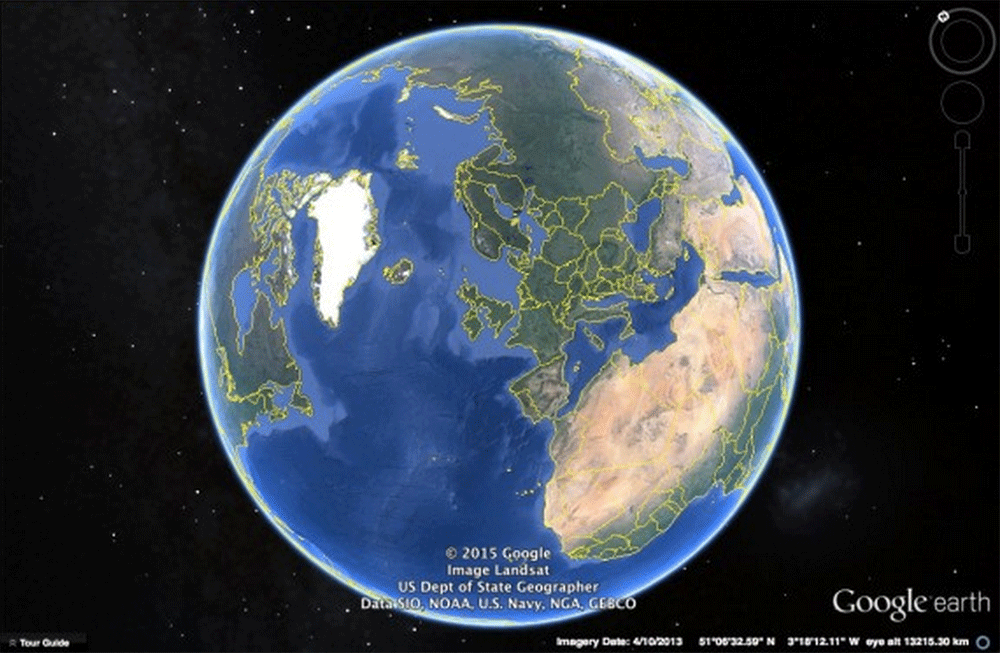
\includegraphics[width=\textwidth,height=\applicationheight]{images/literature/earth-science}
        \caption{Earth science \parencite{google2015earth}}
        % \protect\footnotemark}
        \label{fig:earth_science}
    \end{subfigure}
    \begin{subfigure}[b]{\applicationwidth}
        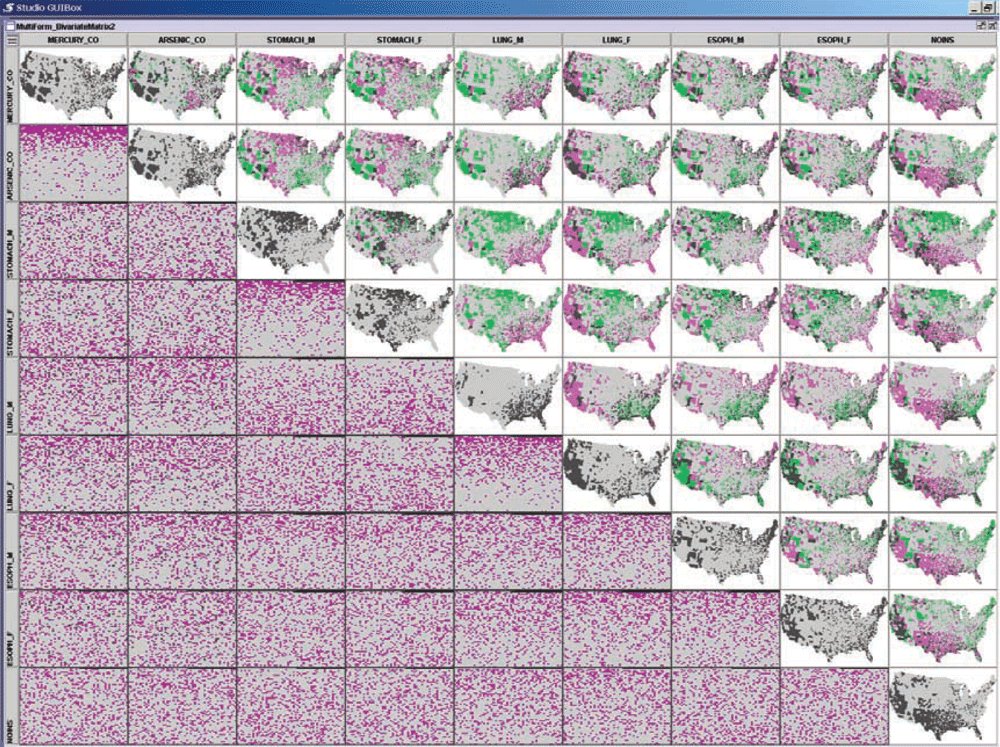
\includegraphics[width=\textwidth,height=\applicationheight]{images/literature/public-health}
        	\caption{\tiny{Public health \parencite{maceachren2004geovisualization}}}
        \label{fig:public_health}
    \end{subfigure}
    \begin{subfigure}[b]{\applicationwidth}
        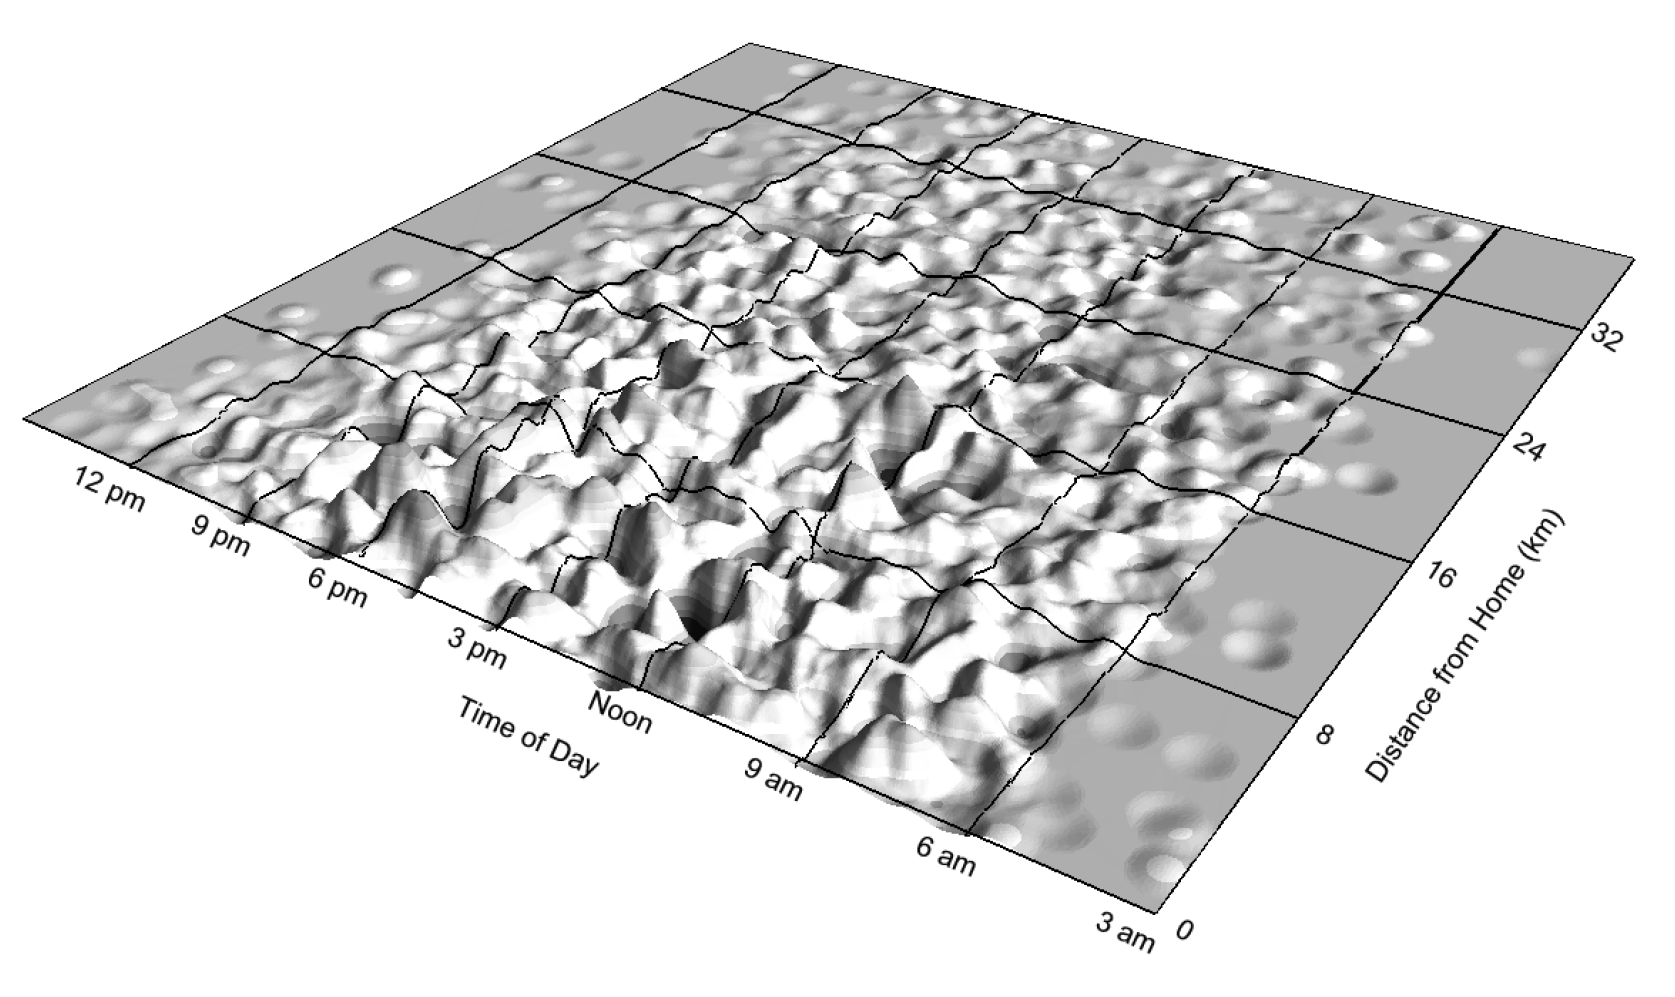
\includegraphics[width=\textwidth,height=\applicationheight]{images/literature/social-science}
        	\caption{Social science \parencite{kwan2004geovisualization}}
        \label{fig:social_science}
    \end{subfigure}
	\caption[Geovisualisation application domains]{Examples of geovisualisations used in various application domains.}
	\label{fig:geovisualisation_applications}
\end{figure}

% \footnotetext{\bibentry{google2015earth}}